\documentclass{article}
\usepackage{xeCJK}
% if you need to pass options to natbib, use, e.g.:
%\PassOptionsToPackage{numbers, compress}{natbib}
% before loading nips_2017
%
% to avoid loading the natbib package, add option nonatbib:
% \usepackage[nonatbib]{nips_2017}

\usepackage[final]{nips_2017}

% to compile a camera-ready version, add the [final] option, e.g.:
% \usepackage[final]{nips_2017}

\usepackage[utf8]{inputenc} % allow utf-8 input
\usepackage[T1]{fontenc}    % use 8-bit T1 fonts
\usepackage{hyperref}       % hyperlinks
\usepackage{url}            % simple URL typesetting
\usepackage{booktabs}       % professional-quality tables
\usepackage{amsfonts}       % blackboard math symbols
\usepackage{nicefrac}       % compact symbols for 1/2, etc.
\usepackage{microtype}      % microtypography
\usepackage{bm}             % bold in math
\usepackage{graphicx}       % images
\usepackage{algorithm}      % algorithm
\usepackage[noend]{algpseudocode} % algorithm
\usepackage{caption}        % captionof
\usepackage{array}          % thick column hline
\usepackage{booktabs}       % table style
\usepackage{pbox}           % table line break
\usepackage{subcaption}     % multiple figures
\usepackage{listings}
\usepackage{xcolor}
\usepackage{tikz}
\usepackage{amsmath}
\definecolor{mygreen}{rgb}{0,0.6,0}
\definecolor{mygray}{rgb}{0.5,0.5,0.5}
\definecolor{mymauve}{rgb}{0.58,0,0.82}
\definecolor{codeBkg}{rgb}{0.85,0.85,0.85}

\lstset{ 
	backgroundcolor=\color{codeBkg},   % choose the background color; you must add \usepackage{color} or \usepackage{xcolor}; should come as last argument
	basicstyle=\footnotesize,        % the size of the fonts that are used for the code
	breakatwhitespace=false,         % sets if automatic breaks should only happen at whitespace
	breaklines=true,                 % sets automatic line breaking
	captionpos=b,                    % sets the caption-position to bottom
	commentstyle=\color{mygreen},    % comment style
	deletekeywords={...},            % if you want to delete keywords from the given language
	escapeinside={\%*}{*)},          % if you want to add LaTeX within your code
	extendedchars=true,              % lets you use non-ASCII characters; for 8-bits encodings only, does not work with UTF-8
	frame=no,	                   % adds a frame around the code
	keepspaces=true,                 % keeps spaces in text, useful for keeping indentation of code (possibly needs columns=flexible)
	keywordstyle=\color{blue},       % keyword style
	language=Octave,                 % the language of the code
	morekeywords={*,...},            % if you want to add more keywords to the set
	numbers=left,                    % where to put the line-numbers; possible values are (none, left, right)
	numbersep=5pt,                   % how far the line-numbers are from the code
	numberstyle=\tiny\color{mygray}, % the style that is used for the line-numbers
	rulecolor=\color{black},         % if not set, the frame-color may be changed on line-breaks within not-black text (e.g. comments (green here))
	showspaces=false,                % show spaces everywhere adding particular underscores; it overrides 'showstringspaces'
	showstringspaces=false,          % underline spaces within strings only
	showtabs=false,                  % show tabs within strings adding particular underscores
	stepnumber=1,                    % the step between two line-numbers. If it's 1, each line will be numbered
	stringstyle=\color{mymauve},     % string literal style
	tabsize=4,	                   % sets default tabsize to 2 spaces
	title=\lstname                   % show the filename of files included with \lstinputlisting; also try caption instead of title
}

\title{量化交易平台开发手册}

\hypersetup{
    colorlinks = true,
}
\makeatletter
\def\BState{\State\hskip-\ALG@thistlm}
\makeatother
\floatname{algorithm}{Procedure}
\renewcommand{\algorithmicrequire}{\textbf{Input:}}
\renewcommand{\algorithmicensure}{\textbf{Output:}}

\newcolumntype{?}{!{\vrule width 3pt}}

\author{
  闫涛 \\
  %% examples of more authors
  %% \And
  %% Nicholas Frosst \\
  %% Affiliation \\
  %% Address \\
  %% \texttt{email} \\
  %% \AND
  %% Geoffrey E. Hinton \\
  阿尔山金融科技有限公司\\
  北京 \\
  \texttt{\{yt7589\}@qq.com} \\
  %% Affiliation \\
  %% Address \\
  %% \texttt{email} \\
  %% \And
  %% Coauthor \\
  %% Affiliation \\
  %% Address \\
  %% \texttt{email} \\
  %% \And
  %% Coauthor \\
  %% Affiliation \\
  %% Address \\
  %% \texttt{email} \\
}
\date{March 2019}

% \usepackage{natbib}
% \usepackage{graphicx}

\begin{document}

\maketitle
\begin{abstract}
基于tushare.org开放数据集,构建本地量化交易开发平台。
\end{abstract}
\section{概述}
\subsection{环境搭建}
创建开源项目,项目网址:https://github.com/yt7589/aqp ,本地环境为:d:/awork/aftdc/incubate/aqp,虚拟环境激活:d:/aadesk/dev/python/quant/Script/activate ,这个是通过python -m venv quant来创建的虚拟环境。
\subsection{整体架构}
app\_main.py:程序主入口; \newline
app\_registry.py:管理程序中所有全局性配置和变量;\newline
controller目录:所有业务逻辑实现类;\newline
model目录:所有数据库操作类;\newline
\subsection{数据服务商}
我们采用的是tushare.pro提供的数据服务:https://tushare.pro 。
\section{数据处理}
数据处理包括从tushare.org网站获取数据,将其转化为量化平台所需的数据格式。
\subsection{获取沪深市场所有挂牌股票}
获取在沪深两市挂牌的所有股票的基本信息。
\subsubsection{接口定义}
获取股票基本信息接口为stock\_basic,其参数为:

\begin{table}[h]
\caption{stock\_basic接口输入参数说明}
\label{t000001}
\begin{tabular}{|c|c|c|c|} \hline
名称 & 类型 & 必选 & 描述 \\ \hline  
is\_hs & str & N & 是否沪深港通标的,N否 H沪股通 S深股通 \\ \hline
list\_status & str & N & 上市状态: L上市 D退市 P暂停上市 \\ \hline
exchange & str & N & 交易所:SSE上交所 SZSE深交所 HKEX港交所 \\ \hline
\end{tabular}
\end{table}

返回值为:
\begin{table}[h]
\caption{stock\_basic接口返回结果说明}
\label{t000002}
\begin{tabular}{|c|c|c|} \hline
名称 & 类型 & 描述 \\ \hline  
ts\_code & str & TS代码 \\ \hline
symbol & str & 股票代码 \\ \hline
name & str & 股票名称 \\ \hline
area & str & 所在地域 \\ \hline
industry & str & 所属行业 \\ \hline
fullname & str & 股票全称 \\ \hline
enname & str & 英文全称 \\ \hline
market & str & 市场类型 (主板/中小板/创业板) \\ \hline
exchange & str & 交易所代码 \\ \hline
curr\_type & str & 交易货币 \\ \hline
list\_status & str & 上市状态: L上市 D退市 P暂停上市 \\ \hline
list\_date & str & 上市日期 \\ \hline
delist\_date & str & 退市日期 \\ \hline
is\_hs & str & 是否沪深港通标的,N否 H沪股通 S深股通 \\ \hline
\end{tabular}
\end{table}


调用格式为:
\lstset{language=PYTHON, caption={获取股票基本信息}, label={c000001}}
\begin{lstlisting}
import tushare as ts
pro = ts.pro_api()
data = pro.stock_basic(exchange='', list_status='L', 
                    fields='ts_code,symbol,name,area,industry,list_date')
data = pro.query('stock_basic', exchange='', list_status='L', 
			fields='ts_code,symbol,name,area,industry,list_date')
\end{lstlisting}
见\ref{c000001}所示
结果示例:
\lstset{language=BASH, caption={获取股票基本信息结果示例}, label={c000002}}
\begin{lstlisting}
    ts_code     symbol     name     area industry    list_date
0     000001.SZ  000001  平安银行   深圳       银行  19910403
1     000002.SZ  000002   万科A   深圳     全国地产  19910129
2     000004.SZ  000004  国农科技   深圳     生物制药  19910114
3     000005.SZ  000005  世纪星源   深圳     房产服务  19901210
4     000006.SZ  000006  深振业A   深圳     区域地产  19920427
5     000007.SZ  000007   全新好   深圳     酒店餐饮  19920413
\end{lstlisting}

\subsubsection{区域信息}
如代码\ref{c000002}所示,地区是以字符串形式返回的。我们可能需要按地区来统计股票表现,因此需要将地区统计出来,放到单独的一个表中进行管理。
\paragraph{数据库设计}
数据库结构表结构如下所示:
\lstset{language=SQL, caption={地区表数据结构}, label={c000003}}
\begin{lstlisting}
create table t_area(
	area_id int primary key auto_increment,
	area_name varchar(200)
);
\end{lstlisting}
\paragraph{信息处理}
当我们读到返回结果的一行时,我们取出地区信息,然后查询t\_area表中是否包含该地区,如果包含则返回对应的area\_id,否则将该地区添加到t\_area表中,并返回其area\_id。
\subsubsection{行业信息}
\paragraph{数据库设计}
\paragraph{信息处理}
\subsubsection{股票信息}
\paragraph{接口定义}
\paragraph{获取并处理数据}
\subsection{获取日线行情数据}
\section{量化模型}
\subsection{时间序列分析}
\section{回测系统}
\subsection{数据库系统设计}
客户是自然人,用t\_customer表示。客户加上账户再加上量化策略,形成我们系统的用户,用t\_user来表示。
账户中具有现金资产和股票资产。
账户具有资金的入和出,有股票的买入和卖出。
用户持有一些股票,可以对股票进行买卖。
用户可以买入和卖出指定数量股票,与账户资金变动相关联
股票参数表:买入费率、印花税;卖出费率、印花税等,计入交易成本中。
\subsubsection{ER图}
\begin{figure}[H]
	\caption{数据库表ER图}
	\label{f000001}
	\centering
	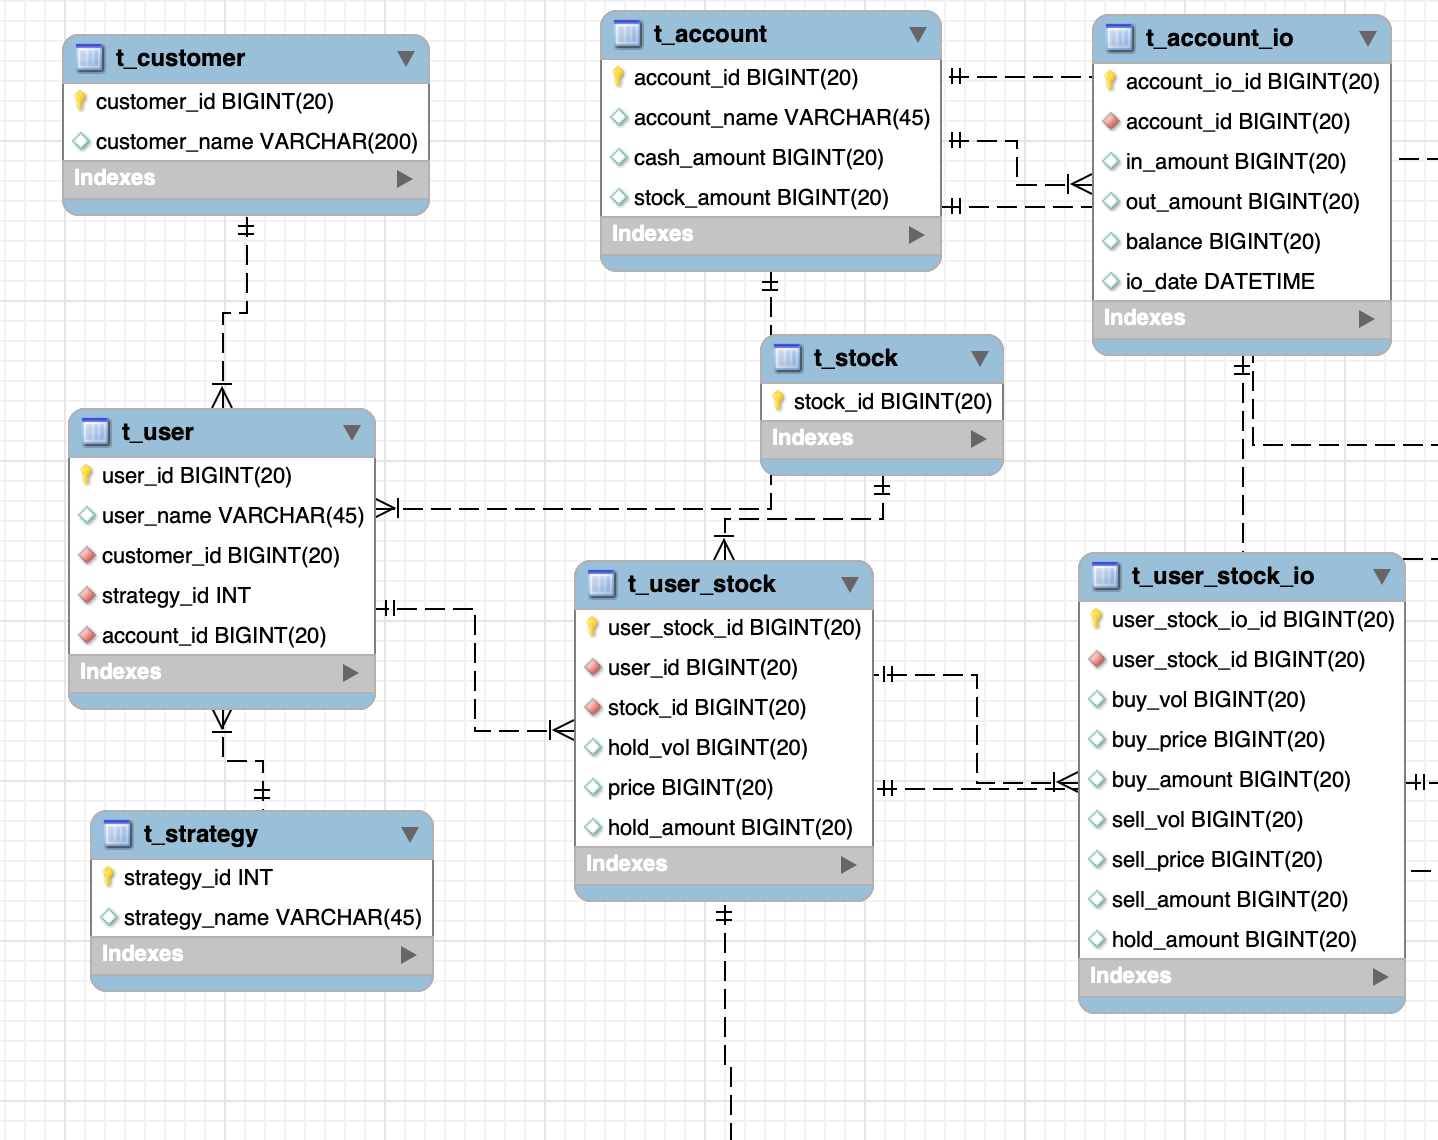
\includegraphics[height=10cm]{images/f000001}
\end{figure}
\subsubsection{客户表}
表示自然人客户,结构如下所示:
\begin{table}[h]
    \caption{客户表(t\_custome)}
    \label{t000001}
    \begin{tabular}{|p{2cm}|p{3cm}|p{2cm}|p{5cm}|} \hline
    字段 & 名称 & 类型 & 描述 \\ \hline 
    customer\_id & 客户编号 & bigint & 主键且自增长 \\ \hline
    customer\_name & 客户姓名 & varchar & 真实姓名 \\ \hline
    \end{tabular}
    \end{table}

参考文献:
\cite{ex1}---\cite{ex2}---\cite{refa001}

\newpage

\bibliographystyle{plainnat}
\bibliography{nips}

\appendix


\end{document}
